\chapter{実装}
\label{chap:implementation}
本章ではRive日本語入力を構成する各システムについて
詳細な実装の解説を行う。

\newpage
\section{Rive Client}
\label{sec:riveclient}
本システムはAndroidOS\footnote[1]{http://www.google.com/intl/ja/mobile/android/}
上で動くアプリケーション
として実装した。
ユーザは本アプリケーションをインストールし、
使用するIMEに選択することで
Rive日本語入力を利用することができる。

\subsection{システムフロー}
このシステムが立ち上がるとまず始めにonCreate()が呼ばれ、初期化を行う。
その後onStartInput()メソッドが呼ばれコンテキストを取得する。
このコンテキストはデバイスの情報を取得する。
コンテキストを取得し次第、候補単語を取得する。
この候補単語はサーバーと通信した上で取得する。
これをユーザーが一つの操作を行うたびに繰り返す。
ここで言う一つの動作とは、キーボード上の一つの文字を押すことや、
候補の単語をタップすること、
あるいは文字をデリートすることも含まれる。
最終的にユーザーが入力を終了した場合にはonFinishInput()が呼ばれ、
今回のユーザが行った動作とコンテキストを紐付けサーバーに送信する。
通信が終わり次第onDestory()が呼ばれ本システムは終了する。
(システムフローイメージ図:\ref{fig:clientflow})
\begin{figure}[htbp]
  \begin{center}
    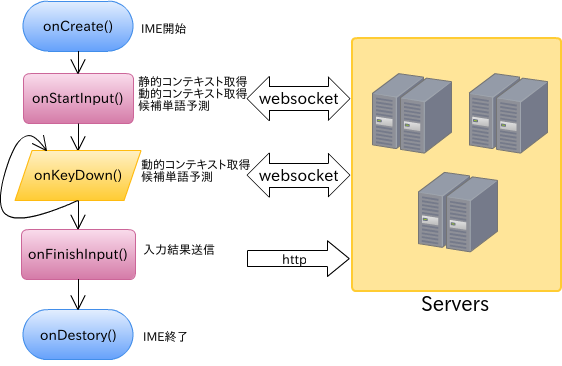
\includegraphics[width=140mm,bb=0 0 562 366]{images/clientflow}
  \end{center}
  \caption{Rive Clientフローイメージ}
  \label{fig:clientflow}
\end{figure}

\subsection{コンテキスト取得}
取得するコンテキストについては\ref{sec:getcontext}項を参照。
コンテキストはユーザーが入力できるものはユーザが入力する。
その他デバイスで取得可能なものを全て取得し、推薦システムに使う。

\section{Rive Server}
\label{sec:riveserver}
VPS上で動かしているサーバー群である。
主に推薦に関する処理を担っている。

\subsection{システム構成}
サーバーの中身は大きくRoutting Server,beforeRules,afterRules,Jubatusの
4つを実装した。
Routing ServerはNode.js\footnote{http://nodejs.jp/}によって実装した。
それぞれ候補単語の計算手法が異なるため(図:\ref{fig:riveserver})
ような分割になっている。
\begin{figure}[htbp]
  \begin{center}
    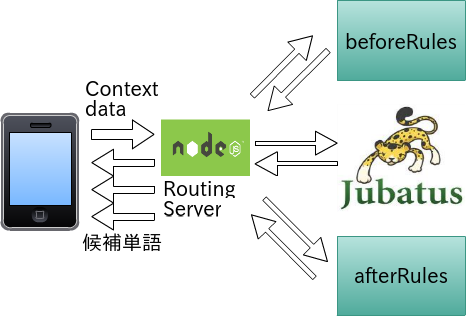
\includegraphics[width=14cm,bb=0 0 466 316]{images/riveserver.png}
  \end{center}
  \caption{Rive Server概要図}
  \label{fig:riveserver}
\end{figure}
始めにクライアントがコンテキストデータをRouting Serverへ送信する。
その後Routing ServerがbeforeRulesへコンテキストデータを送る。
beforeRulesは送られてきたデータを元に推薦候補単語をRouting Serverに送る。
Routing Serverは受け取ったデータをクライアントに返すと共に、
Jubatusへコンテキストデータを再送する。
Jubatusはそのデータを元に推薦候補単語を推測しRouting Serverへ送る。
Routing Serverは受け取ったデータを更にクライアントへ送る。
そしてそれと共にコンテキストデータをafterRulesに再送する。
そのデータを元に推薦候補単語をRouting Serverへ送る。
そしてそれをクライントに返すことで完了する。
一回のタッチごとにこれら全てのプロセスを行う。
またこれらの一度の過程ごとにユニークなIDをつけてあり、
途中で新しいプロセスが始まった場合前のプロセスは破棄されることで
常に最新の推薦候補単語を受け取ることができる。

\subsection{Routing Server}
このサーバーはふたとおりの役割を持っている。
一つはデバイスから受け取ったコンテキストデータを
beforeRules,Jubatus,afterRulesの3つの計算エンジンに振り分け送信する役割である。
もうひとつは受け取ったデータを受け取り次第、デバイスに送信する役割である。

\subsection{beforeRules}
\label{sec:beforerules}
このエンジンはコンテキストデータが送られてきた際に、
一定のルールに基づいているものをまとめている。
このルールは開発者がよく使う単語を推測し実装した。
例えば、Twitter\footnote{http://twitter.com/}
クライアントに入力を行っている(行おうとしている)
場合に「なう」「@」の候補単語を返すようになっている。

\subsection{Jubatus}
このエンジンについては第\ref{sec:jubatus}項参照。

\subsection{afterRules}
\label{sec:afterrules}
このエンジンはbeforeRulesより重要度が低く、
また計算に時間がかかるものを推測して実装した。
例えば、最寄り駅をクエリとしてその駅を通っている電車の線を
その場でWEBから検索し推薦単語として返すことができる。

\section{Rive Analytics}
このシステムはRive Client\ref{sec:riveclient}でのプロセスの終わりに
送られてくるデータを受信し、解析するシステムである。
開発者はこのシステムを使用することによって、新しい機能の有用性などを
確かめることができる。

\subsection{指標値に用いる単語の説明}
\begin{description}
  \item[click] タッチ
  \item[touch] 候補単語のタッチ
  \item[before] beforeRules(\ref{sec:beforerules}項)からのタッチ
  \item[after] afterRules(\ref{sec:afterrules}項)からのタッチ
  \item[jubatus] Jubatus(\ref{sec:jubatus}項)からのタッチ
  \item[recommend] beforeRulesとafterRulesとJubatusの総和からのタッチ
  \item[score] Jubatusにおいて算出したスコア
\end{description}
\subsection{指標値}
\begin{itemize}
  \item CPI - Click Per Input\mbox{}\\
    この指標値は一度の入力に対して
    平均でどれくらいクリックしたかを示している値である。
    値を低く保つことで入力の省入力化を達成できる。
  \item msPI - milliseconds Per Input\mbox{}\\
    この指標値は一度の入力に対して
    平均で何ミリ秒かかったかを示している値である。
    値を低く保つことで入力の少入力かを達成できる。
  \item TPI - Touch Candidate Per Input\mbox{}\\
    この指標値は一度の入力に対して
    平均で何度候補単語をタッチしたかを示している値である。
    推薦エンジンの有用性を示す値となる。
  \item TPC - Touch Candidate per Click\mbox{}\\
    この指標値はクリック回数のうち
    候補単語がタッチされた割合を示す値である。
    割合を把握することで、
    キーボードと候補のどちらを改善すべきかを示す値である。
  \item RPC - Recommend Per Touch\mbox{}\\
    この指標値は候補単語をタッチされた回数のうち
    どれだけの割合で推薦候補をタッチされたかを示す値である。
    この値を高めることで推薦エンジンの有用性を示す。
  \item Score - Score average by Jubatus\mbox{}\\
    この指標値はJubatusによる推薦単語がタッチされた時に、
    いくつのスコアのものがタッチされたかを示す値である。
    beforeRulesやafterRulesの閾値の参考にする値である。
  \item BPR - BeforeRules Per Recommend\mbox{}\\
    この指標値は推薦単語がタッチされたうちの
    beforeRulesのタッチされた割合を示す値である。
    beforeRulesの有用性を示す値となる。
  \item APR - AfterRules Per Recommend\mbox{}\\
    この指標値は推薦単語がタッチされたうちの
    afterRulesのタッチされた割合を示す値である。
    afterRulesの有用性を示す値となる。
  \item JPR - Jubatus Per Recommend\mbox{}\\
    この指標値は推薦単語がタッチされたうちの
    Jubatusからきた推薦単語のタッチされた割合を示す値である。
    Jubatusからくる推薦単語の有用性を示している。
  \item JPT - Jubatus Per Touch\mbox{}\\
    この指標値は候補単語をタッチした回数のなかで
    Jubatusからくる推薦単語の割合を示す値である。
    jubatusからくる推薦単語の有用性を示している。
\end{itemize}
これらをgitのcommitとひもづけることによってバージョンごとに
データを管理している。(図:\ref{fig:riveanalytics})
\begin{figure}[htbp]
  \begin{center}
    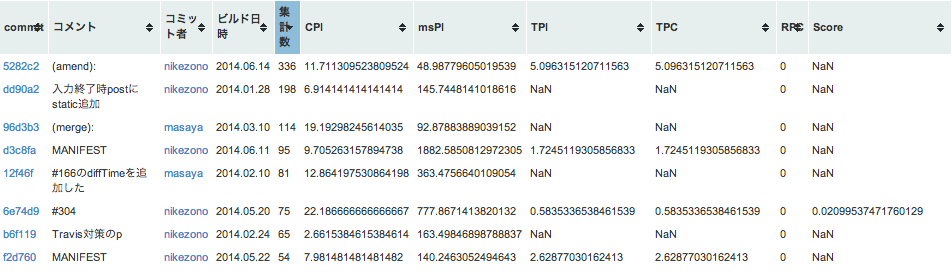
\includegraphics[width=170mm,bb=0 0 952 274]{images/riveanalytics.png}
    \caption{Rive Analytics画面}
    \label{fig:riveanalytics}
  \end{center}
\end{figure}

\section{Rive Batchprocessing}
このシステムは定期的に処理を行うものを管理し実行している。
インターネット上のデータをクロールし、
DBを定期的にアップデートするプログラムなどが構成している。

\section{Rive Webservice}
このシステムはインターネット上で閲覧可能なホームページとして実装した。
Rive ServerとRive Webserviceは通信を行い、
仮想のコンテキストを作り出すことで
推薦の状態を確かめることができる。
(体験画面イメージ:\ref{fig:rivewebservice})
\begin{figure}[htbp]
  \begin{center}
    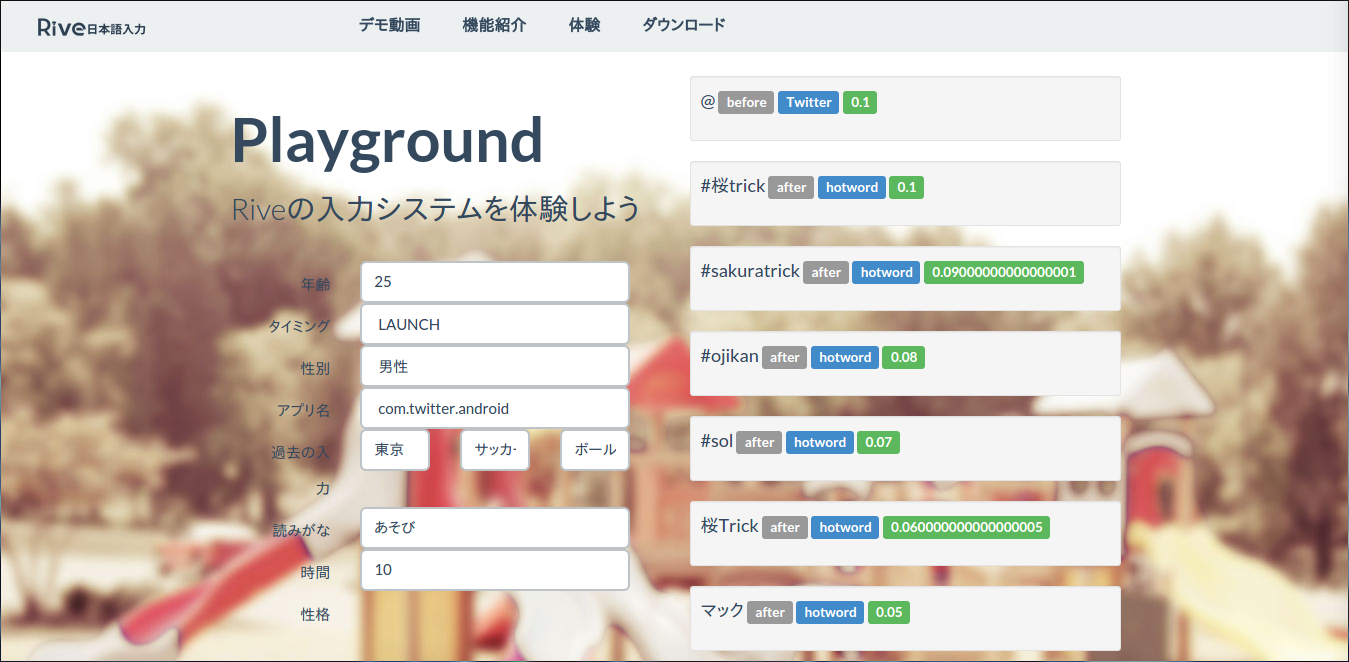
\includegraphics[width=160mm,bb=0 0 1349 662]{images/rivewebservice.png}
    \caption{Rive Webserviceの体験画面}
    \label{fig:rivewebservice}
  \end{center}
\end{figure}

